%!TEX root = ../dissertation.tex

\chapter{Implementation}
\label{chapter:implementation}

The application developed follows a Model-View-Controller architecture.

This architecture is composed of three elements \cite{krasner1988description}:
\begin{itemize}
\item The Model, which captures and stores information about the application domain;
\item The View, which generates output based on the model state;
\item The Controller, which provides interaction between the Views and the Model. It is able to modify the Model and update the corresponding View.
\end{itemize}

The standard interaction cycle in this architecture is the following \cite{krasner1988description,reenskaug2009dci}:
\begin{itemize}
\item A user interacting with the application sends a request to the Controller.

\item The Controller communicates with the Model to apply the desired changes.

\item The Model is updated.

\item The Controller notifies the corresponding View so it can be updated with the new version of the Model.
\end{itemize}

The next sections will describe the solution implementation based on these three elements.


\section{Model}
\label{section:model}
The Model of the implemented system is based on the Domain Model presented in chapter \ref{chapter:domainModel}, but a few modifications were made to facilitate programming.

The developed application uses the F\'{e}nix Framework, which allows the creation of a transactional and persistent domain model for applications \cite{cachopo2006combining,cachopo2007development}. The domain model is specified in the Domain Modeling Language, which is a domain-specific language created for this framework. The framework completely hides the database from the programmer, who can focus on the application development in Java. 

\subsection{Annotations}
\label{subsection:modelAnnotations}
As seen in Chapter \ref{chapter:architecture}, the Document is one of the most important entities, because it aggregates all the annotations created over the text and all the Software Architectures concepts elicited.

Similarly to what is shown in Figure \ref{figure:documentAnnotationConcepts} of Chapter \ref{chapter:architecture}, in the implemented model, the Document entity is connected to the Annotation. However, an annotation is created by an user authenticated in the system, and this information is also present in the domain, as shown in figure \ref{figure:modelDocUserAnnot}. The ``User'' entity saves users registered in the system. When a user creates an annotation, it is associated to him.

\begin{figure}
\centering
\renewcommand {\umltextcolor}{black}
\renewcommand {\umlfillcolor}{none}
\renewcommand {\umldrawcolor}{black}

\begin{tikzpicture}
\tikzstyle{every node}=[font=\footnotesize]
\begin{class}[text width=3cm ]{Document}{0,0}
	\attribute { title : String }
	\attribute { url : String }
	\attribute { content : String }
\end{class}

\begin{class}[text width=3.5cm ]{Annotation}{-2,-5}
	\attribute { annotation : String }
	\attribute { tag : String }
\end{class}

\begin{class}[text width=3.5cm ]{User}{-6,0}
	\attribute { username : String }
	\attribute { password : String }
	\attribute { firstName : String }
	\attribute { lastName : String}
	\attribute { type : String}
\end{class}
\association {Document}{document}{1}{Annotation}{annotation}{0..*}
\association {User}{owner}{1}{Annotation}{annotation}{0..*}

\end{tikzpicture}
\caption{Document, Annotations and Users in the implemented Model}
\label{figure:modelDocUserAnnot}
\end{figure} 
 
\subsection{Scenarios}
\label{subsection:modelScenarios}
The Scenario is a main concept of the domain, and therefore is connected to the Document, as seen in Figure \ref{figure:documentConcept}. 

Scenarios are represented in the implemented model in a very similar way to what is shown in Figure \ref{figure:abstractDomainModel}. However, there is a difference in the implemented model regarding how Quality Requirements and Tactics are represented.

In Figure \ref{figure:abstractDomainModel}, it is shown an association between Scenario and Quality Requirement, Scenario and Tactic and Tactic and Quality Requirement. The meaning of these associations is to represent what is explained in Section \ref{subsection:SAConceptsScenarios}: A Scenario has a Quality Requirement from a set of pre-existent ones, and a set of Tactics also from a set of existent ones, which are specific for the Quality Requirement.

However, in the implemented model, there are no pre-existent Tactics nor Quality Requirements. The existent Quality Requirements and their specific Tactics are specified in a Java class, which returns them as necessary. Figure \ref{figure:modelQRTactics} shows the Scenario, Tactic and Quality Requirement entities, and how they are related in the implemented model.

\begin{figure}[h]
\centering
\renewcommand {\umltextcolor}{black}
\renewcommand {\umlfillcolor}{none}
\renewcommand {\umldrawcolor}{black}

\begin{tikzpicture}
\tikzstyle{every node}=[font=\footnotesize]
\begin{class}[text width=3cm ]{Scenario}{0,0}
	\attribute { name : String}
	\attribute { identifier : String }
	\attribute { text : String }
\end{class}

\begin{class}[text width=3cm ]{QualityRequirement}{-5,0}
	\attribute { name : String}
\end{class}

\begin{class}[text width=3cm ]{Tactic}{-5,-2}
	\attribute { identifier : String }
	\attribute { text : String }
\end{class}

\association {Scenario}{}{1}{Tactic}{}{*}
\association {Scenario}{}{0..1}{QualityRequirement}{}{0..1}

\end{tikzpicture}
\caption{Quality Requirements and Tactics detail in the implemented Model}
\label{figure:modelQRTactics}
\end{figure}

To create a Scenario, it is necessary to select a Quality Requirement from a list, which is retrieved from the class mentioned. When the Scenario is created, a new Quality Requirement is also created, with the selected one stored into the ``name'' attribute, and associated with that Scenario. Tactics can be added once inside the Scenario Template. To add a tactic it is necessary to select it from a list of specific tactics for the quality requirement. That list is, again, retrieved from the class mentioned before. When a specific tactic is selected, a new Tactic is created in the model with the specific tactic name stored in the ``identifier'' attribute. Given these implementation details, there was no need to create the association between Tactic and QualityRequirement nor to have a Quality Requirement associated with many Scenarios.

To facilitate programming, all Scenario elements are a subclass of a ``ScenarioElement'' class, as seen in the example in Figure \ref{figure:modelScenarioElement}. This superclass aggregates all the methods common to the Scenario elements, making it easier to perform actions such as updating the text, associating annotations or presenting the elements in a view. A few of those methods are shown in the figure. However, this class is not associated with the Scenario entity. Its purpose is only to facilitate programming by aggregating common methods. 

\begin{figure}[h]
\centering
\renewcommand {\umltextcolor}{black}
\renewcommand {\umlfillcolor}{none}
\renewcommand {\umldrawcolor}{black}

\begin{tikzpicture}
\tikzstyle{every node}=[font=\footnotesize]
\begin{class}[text width=3cm ]{ScenarioElement}{0,0}
	\attribute { identifier : String }
	\attribute { text : String }
	\operation { getIdentifier() : String }
	\operation { getText() : String}
	\operation { (...)}
\end{class}

\begin{class}[text width=2.5cm ]{SrcOfStimulus}{-2.1,-4}
	\inherit{ScenarioElement}
	\attribute{}
\end{class}

\draw [umlcd style] (0,-4.3) node {[...]};

\begin{class}[text width=3cm ]{ResponseMeasure}{2.2,-4}
	\inherit{ScenarioElement}
	\attribute{}
\end{class}		
	
\end{tikzpicture}
\caption{The ScenarioElement entity}
\label{figure:modelScenarioElement}
\end{figure}

The ``identifier'' parameter of the entities, seen in Figures \ref{figure:modelQRTactics} and \ref{figure:modelScenarioElement} stores the name of the concept that corresponds to that entity, and often corresponds to the name of the entity itself. For example, the identifier in all instances of Scenario is ``Scenario'' and the identifier in all instances of ``SrcOfStimulus'' is ``Source Of Stimulus''. This was done to facilitate certain programming issues such as getting the concept name from a ``ScenarioElement'' instance. The ``name'' attribute in the Scenario gives it an identification other than just the quality attribute, and the ``text'' attribute in the Scenario and ScenarioElement corresponds to the description text that can be added to the templates.

All domain entities have associated annotations, as it was mentioned previously in Section \ref{section:annotation}. The implemented model is similar to what is shown in Figure \ref{figure:documentAnnotationConcepts}, with the Scenario and ScenarioElement entities being associated with the Annotation.


\subsection{Modules}
\label{subsection:modules}

The Modules are the elements of the Module Viewtype Views. Figure \ref{figure:modelModule} shows how a Module is represented in the implemented model.

\begin{figure}[h]
\centering
\renewcommand {\umltextcolor}{black}
\renewcommand {\umlfillcolor}{none}
\renewcommand {\umldrawcolor}{black}

\begin{tikzpicture}
\begin{class}[text width=3cm ]{Module}{0,0}
	\attribute { name : String }	
	\attribute { identifier : String }
	\attribute { text : String }
\end{class}			
\end{tikzpicture}
\caption{The Module entity}
\label{figure:modelModule}
\end{figure}

The Module entity has a ``name'' attribute, which provides identification and also gives an idea on what are the Module functions, an ``identifier'', as explained in the previous section, and a ``text'' attribute, which corresponds to text added to the template.

As it is one of the main concepts of the system, the Module is associated with the corresponding document upon its creation as demonstrated in the example in Figure \ref{figure:documentAnnotationConcepts}. The Module is also associated with the set of Annotations that describe it.

As seen in the abstract domain model present in Figure \ref{figure:abstractDomainModel} of Chapter \ref{chapter:domainModel}, the elements of a view have a certain type of relationship with each others. Although the abstract domain model in Figure \ref{figure:abstractDomainModel} contains an entity ``Relation'' to represent how the view elements are connected, in the case of the Modules, these relations have no other information than the Modules connected. 

Therefore, in the implemented model, there are no entities representing the relationships between modules. Instead, there were defined different associations of the Module entity to itself, in order to represent the different relations.

Each Module Viewtype Style specifies relation types refined from the ones presented in \ref{subsection:domainModelViews}. There are, then, eight types of relations between Modules\cite{clements2003documenting} defined in the Domain Modeling Language:
\begin{itemize}
\item \textit{Is-Part-Of} - a Module can be part of one and only one parent Module. Figure \ref{figure:modelIsPartOfRelation} shows how this relation was implemented. A Module can have only one other Module set as parent, but can have many children Modules;
\begin{figure}[h]
\centering
\lstset{style=customjava}
\begin{tabular}{c}
\begin{lstlisting}
relation moduleIsPartOfModule {
	Module playsRole parent{ multiplicity 0..1; }
	
	Module playsRole child{ multiplicity 0..*; }
}
\end{lstlisting}
\end{tabular}
\caption{Is-Part-Of relation between Modules in the implemented model}
\label{figure:modelIsPartOfRelation}
\end{figure}

\item \textit{Uses} - a specialization of the \textit{depends-on} relation, where a Module depends on the correct functioning of other Modules to satisfy its own requirements. The implementation is shown in Figure \ref{figure:modelUsesRelation}. A Module can use and be used by many other Modules;
\begin{figure}[h]
\centering
\lstset{style=customjava}
\begin{tabular}{c}
\begin{lstlisting}
relation moduleUsesModule {
	Module playsRole uses{ multiplicity 0..*; }
	
	Module playsRole usedBy{ multiplicity 0..*; }
}
\end{lstlisting}
\end{tabular}
\caption{Uses relation between Modules in the implemented model}
\label{figure:modelUsesRelation}
\end{figure}

\item \textit{Is-A} - a relation of generalization, in which a Module is a generalization, similar to a superclass, of other modules. The implementation of this relation is similar to the implementation of the ``Uses'' relation in Figure \ref{figure:modelUsesRelation}, as a Module can be a generalization of many Modules and a specialization of many others (multiple inheritance).

\item \textit{Crosscuts} - an Aspect Module, which implements a crosscutting concern of the system, is bound to a Module that is affected by that crosscutting concern. The Implementation of this relation is similar to the one shown in Figure \ref{figure:modelUsesRelation}, as a Module can be a crosscutting concern of many Modules, and be crosscutted by other Aspect Modules.

\item \textit{One-To-One, One-To-Many, Many-to-Many} - logical associations between Data Entity Modules, similar to the UML associations. The implementation of these relations is, again, similar to the implementation of the ``Uses'' relation in Figure \ref{figure:modelUsesRelation}. The '0..*' cardinality in the one-to-one, one-to-many and many-to-many relations means that a Module can have several relations of this type in a Data Model Style view. For example, if a Module instance with name ``Department'' has a ``One-To-Many'' relation with Modules ``Employee'' and ``Room'', it means that a visual representation of these Modules would be the one in figure \ref{figure:modelOneToManyExample}.
\begin{figure}[h]
\centering
\renewcommand {\umltextcolor}{black}
\renewcommand {\umlfillcolor}{none}
\renewcommand {\umldrawcolor}{black}
\begin{tikzpicture}
\tikzstyle{every node}=[font=\footnotesize]
\begin{class}[text width=2.5cm ]{Department}{0,0}
	\attribute {}
\end{class}

\begin{class}[text width=2cm ]{Room}{-2.5,-2}
	\attribute {}
\end{class}

\begin{class}[text width=2cm ]{Employee}{2.5,-2}
	\attribute {}
\end{class}

\association{Department}{}{1}{Room}{}{*}
\association{Department}{}{1}{Employee}{}{*}
\end{tikzpicture}
\caption{Example of the One-To-Many relation between Modules}
\label{figure:modelOneToManyExample}
\end{figure}

\item \textit{Aggregation} - an aggregation relation. The implementation of this relation is similar to Figure \ref{figure:modelUsesRelation}, as a Module can be an aggregator of other several Modules, and be aggregated by many others;
\end{itemize}

\subsection{Components and Connectors}
\label{subsection:modelComponentsConnectors}
Components and Connectors are the elements of the Component \& Connector Viewtype Views. Figure \ref{figure:modelComponentConnector} shows how these concepts are represented in the implemented model.

\begin{figure}[h]
\centering
\renewcommand {\umltextcolor}{black}
\renewcommand {\umlfillcolor}{none}
\renewcommand {\umldrawcolor}{black}
\begin{tikzpicture}
\tikzstyle{every node}=[font=\footnotesize]
\begin{class}[text width=2cm ]{Component}{0,0}
	\attribute {name : String}
	\attribute {text : String}
\end{class}

\begin{class}[text width=2cm ]{Connector}{3,0}
	\attribute {name : String}
	\attribute {style : String}
	\attribute {text : String}
\end{class}

\begin{class}[text width=2cm ]{Port}{0,-3}
	\attribute {name : String}
	\attribute {text : String}
\end{class}

\begin{class}[text width=2cm ]{Role}{3,-3}
	\attribute {name : String}
	\attribute {text : String}
\end{class}

\association{Component}{}{0..1}{Port}{}{*}
\association{Connector}{}{0..1}{Role}{}{*}

\end{tikzpicture}
\caption{Component and Connector entities in the implemented model}
\label{figure:modelComponentConnector}
\end{figure}
 
A Component has a set of Ports, and a Connector as a set of Roles. The Ports of a Component are connected to the Roles of a Connector by the \textit{Attachment} relation explained in Section \ref{section:SAConcepts} of Chapter \ref{chapter:domainModel}. The implementation of this relation will be explained further on. The ``name'' and ``text'' attributes in the entities correspond to the identification name of the entity and the descriptive text that can be added, respectively. The ``style'' attribute in the Connector refers to the Component \& Connector styles. Each style has a unique type of connector. Specifying the style of a connector will make it easier to figure which Components will attach to it.

The Component and Connector are main concepts of the system, and therefore are associated with the corresponding document upon creation. Both the Component and Connector entities and also the Port and Role are associated to a set of Annotations that describe them. The associations of these entities to the Document and Annotation are similar to the ones in the example of Figure \ref{figure:documentAnnotationConcepts}.

Components are related with Connectors by the \textit{Attachment} relation. A Component has, as mentioned, a set of ports, and these ports can be attached to roles of Connectors.

Similar to the Module relations, the \textit{Attachment} relation in the implemented model has no more information than the Port and Role involved. Therefore, it did not make sense to create an entity to represent this relation. Instead, a new relation between the Port and Role entity is created in the Domain Modeling language, as shown in Figure \ref{figure:modelAttachmentRelation}.

\begin{figure}[h]
\centering
\lstset{style=customjava}
\begin{tabular}{c}
\begin{lstlisting}
relation portIsAttachedToRole {
	Port playsRole port { multiplicity 0..1; }
	
	Role playsRole role { multiplicity 0..1; }
}
\end{lstlisting}
\end{tabular}
\caption{Attachment relation between Component Ports and Connector Roles in the implemented model}
\label{figure:modelAttachmentRelation}
\end{figure}


\subsection{Views}
\label{subsection:modelViews}

The abstract domain model presented in Figure \ref{figure:abstractDomainModel} of Chapter \ref{chapter:domainModel} shows how a View is related to the Viewtype, the Styles and the elements. 

A View is, as the Scenario, the Element and the Relation, considered a main concept, and therefore has its own dedicated template. Figure \ref{figure:modelView} shows how the View is represented in the implemented model.

\begin{figure}[h]
\centering
\renewcommand {\umltextcolor}{black}
\renewcommand {\umlfillcolor}{none}
\renewcommand {\umldrawcolor}{black}
\begin{tikzpicture}
\begin{class}[text width=3cm ]{View}{0,0}
	\attribute {name : String}
	\attribute {viewtype : String}
	\attribute {text : String}
\end{class}
\end{tikzpicture}
\caption{View entity in the implemented model}
\label{figure:modelView}
\end{figure}

In the abstract domain model of Figure \ref{figure:abstractDomainModel} the View is associated with the Viewtype entity which, in turn, is associated with a Style entity. Similar to what was explained for the Scenarios with the Quality Requirements and Tactics, the abstract domain model assumes there are a set of pre-defined Viewtype entities, each associated with a pre-defined set of Styles. 

In the implemented domain model, however, there are no pre-defined Styles nor Viewtypes. When a view is added to the system, a viewtype must be chosen, and it is stored in the ``viewtype'' attribute. This attribute is used to distinguish what kind of elements can be added to the view. For example, if the ``viewtype'' attribute of a View is set to ``Module Viewtype'', then only Modules are added to that View. 

The styles of a view are not explicitly stated, but they are implicit by the elements that are added to the View. For example, a Module Viewtype View containing a set of Modules with ``uses'' relations between each others implies that there is a \textit{Uses} style in the view, and a Component \& Connector Viewtype View containing Components attached to Connectors with a certain style implies that that style is present in the view. This verification is done by the Controller, as described in Subsection \ref{substection:viewController}.

A View is composed by a set of Elements, as seen in Figure \ref{figure:abstractDomainModel}. In the implemented domain model, the View has a similar association with the Module, Component and Connector entities. Figure \ref{figure:modelviewelements} shows how these relations are implemented in the Domain Modeling Language.

\begin{figure}[h]
\centering
\lstset{style=customjava}
\begin{tabular}{c}
\begin{lstlisting}
relation viewHasModules {
	View playsRole view { multiplicity 0..*; }
	Module playsRole module { multiplicity 0..*;}
}

relation viewHasComponents {
	Component playsRole component { multiplicity 0..*; }
	View playsRole view { multiplicity 0..*; }
}

relation viewHasConnectors {
	Connector playsRole connector { multiplicity 0..*; }
	View playsRole view { multiplicity 0..*; }
}
\end{lstlisting}
\end{tabular}
\caption{Relation between View and the view elements: Module, Component and Connector}
\label{figure:modelviewelements}
\end{figure}

A View is created by associating an Annotation with it and, as it is a main concept, it is associated with the respective Document, as demonstrated in the example in Figure \ref{figure:documentAnnotationConcepts}.

\section{Controller}

This section describes the Controller part of the implemented system. The application developed uses the Spring\footnote{https://spring.io/} Framework, which allows the definition of one or more Java classes to act as Controllers and handle requests.

A Java class is set to be a Controller by annotating it with the \textit{@Controller} annotation, or \textit{@RestController} if the controller's goal is to provide a REST API. Figure \ref{figure:springController} shows an example from the Document Controller described in \ref{subsection:documentController}, with a method that handles requests for the URL \textit{'/selectDoc/{id}'}. Method \textit{showDocument()} retrieves the Document from the domain model with the specified \textit{id} and adds it and the \textit{id} itself as Model attributes, so the template will be able to use them. The template ``docTemplate'' will be then showed to the user.

\begin{figure}[h]
\centering
\lstset{style=customjava}
\begin{tabular}{c}
\begin{lstlisting}
@Controller
public class DocumentController {
	// ...
	@RequestMapping(value = "/selectDoc/{id}", method = RequestMethod.GET)
	public String showDocument(@PathVariable String id, Model m) throws IOException {
		m.addAttribute("docId", id);
		Document d = FenixFramework.getDomainObject(id);
		m.addAttribute("doc", d);
		return "docTemplate";
	}
}	
\end{lstlisting}
\end{tabular}
\caption{Example of a Controller class defined using the Spring Framework} 
\label{figure:springController}
\end{figure}

\subsection{Annotation Controller}
The AnnotationController class provides a way to manage the annotations added to a document. It communicates with the Domain Model to create, remove or update Annotations. This controller is in fact a RestController, which means it provides a REST API, used to retrieve a JSON representation of the annotations stored in the model and display it along with the document text. 
The endpoints provided by this controller are described in Table \ref{table:endpoints}.
	
\begin{table}[h]
\begin{tabular}{ | c | m{1.5cm} | m{3.5cm} |m{7.7cm}|}
    \hline
    \textbf{Name} & \textbf{Request} \textbf{Method }& \textbf{Endpoint} & \textbf{Description}\\ \hline
	INDEX & GET & \parbox[c][1.5cm]{3.5cm}{/selectDoc/\{docId\}/\\store/annotations} & \parbox[c]{8cm}{Returns the set of annotations associated with the \\document with id \textit{docId} }\\ \hline
   	READ & GET & \parbox[c][1.5cm]{3.5cm}{/selectDoc/\{docId\}/\\store/annotations/\{id\}} & Returns the annotation with the specific \textit{id} \\ \hline
    CREATE & POST & \parbox[c]{3.5cm}{/selectDoc/\{docId\}/\\store/annotations} & \parbox[c][1.5cm]{8cm}{Creates a new annotation, stores it in the model \\associated with the document with id \textit{docId}, \\ and redirects to the Read endpoint} \\ \hline
    UPDATE & PUT & \parbox[c][1.5cm]{3.5cm}{/selectDoc/\{docId\}/\\store/annotations/\{id\}} & \parbox[c]{8cm}{Updates the annotation with the given \textit{id} and \\redirects to the READ endpoint} \\ \hline
    DELETE & DELETE & \parbox[t]{3.5cm}{/selectDoc/\{docId\}/\\store/annotations/\{id\}} & \parbox[c][2cm]{8cm}{Removes the association between the \\ annotation with the given id and the document \\ with id \textit{docId}. The response is a HTTP/1.0 204 \\ NO CONTENT.} \\ \hline
  \end{tabular}
  \caption{REST API provided by the Annotation Controller}
  \label{table:endpoints}
\end{table}

The \textbf{INDEX} endpoint has the particularity of iterating through all the Annotations associated with the Document with id \textit{docId}. If the annotation is associated to another domain entity besides the Document (for example, a Scenario, or a Module), information about the domain entity will be added to the annotation body, and will be shown in the interface. This way, it is possible to have some information about the domain entity even before checking its template. 

Figure \ref{figure:annotationControllerIndex} shows an example of how information is added to the annotation in the \textit{INDEX} endpoint. The method \textit{getAnnotations()}, which receives the requests for this endpoint, iterates over the annotations associated with the document with id \textit{docId}, parses the JSON of each annotation into an instance of the AnnotationJS class, checks which domain element is associated with the annotation and adds information accordingly to the field ``text'' of the annotation. The example in the figure shows how information about the viewtype is added to annotations connected with a View. The list of all retrieved AnnotationJS instances is then parsed into a JSON string and sent as response.

\begin{figure}[h]
\centering
\lstset{style=customjava}
\begin{tabular}{c}
\begin{lstlisting}
	@RequestMapping(value = "/selectDoc/{docId}/store/annotations", 
	method = RequestMethod.GET)
	
	public String getAnnotations(@PathVariable String docId) {
		Document d = FenixFramework.getDomainObject(docId);
		List<AnnotationJ> anns = new ArrayList<AnnotationJ>();
		Gson g = new Gson();
		for(Annotation a : d.getAnnotationSet()) {
			AnnotationJ ann = g.fromJson(a.getAnnotation(), AnnotationJ.class);
			if(a.isViewAnnotation() && a.getView() != null) {
				View v = a.getView();
				ann.setText("View: " + v.getViewtype());
			}
			//...			
			anns.add(ann);
		}
		String resp = g.toJson(anns);
		return resp;
	}		
\end{lstlisting}
\end{tabular}
\caption{Example of how the INDEX endpoint adds information to the annotation body}
\label{figure:annotationControllerIndex}
\end{figure}

\subsection{Document Controller}
\label{subsection:documentController}
The DocumentController class handles the requests to view, add or remove a document from the system.

Adding and removing documents from the system is a feature that only Teachers are authorized to use. The controller receives a POST request containing the URL to the article. The Java library JSoup\footnote{http://jsoup.org/} extracts the HTML from the given URL and the controller processes it and stores a Document in the database. Processing of the extracted HTML includes turning relative URLs into absolute ones for href and src attributes.
The Controller will also check if the database already contains a document with the given URL before adding a new entry. 

When a teacher removes a Document from the system, all Annotations and Domain Model entities associated with that Document such as Scenarios or Views are removed from the system as well.

Upon Document visualization, there are three other operations handled by this controller:

\begin{itemize}
\item When a user wants to associate an Annotation with a domain entity such as a Scenario, a request is sent to the Document Controller containing information about the annotation unique ID and its tag. Based on the tag, the controller then redirects to another controller, which will provide means for the user to add and/or select an entity to associate with the annotation.

The reason for this redirect is the existent of a logic division of the Controllers. Each Controller class handles a set of requests related with a certain entity of the domain model. The AnnotationController class handles operations over Annotations, the ScenarioController handles operations over Scenarios and their elements, etc. 

Therefore, it's only logical to redirect this request to the Controller that handles operations over the respective domain entity. Figure \ref{figure:documentControllerLinkAnnotation} shows the method in DocumentController that performs the redirect.

\begin{figure}[h]
\centering
\lstset{style=customjava}
\begin{tabular}{c}
\begin{lstlisting}
	@RequestMapping(value = "/addAnnotationToStructure/{docId}/{annotationId}/{tag}")
	public RedirectView addAnnotationModal(@PathVariable String docId,
			@PathVariable String annotationId, @PathVariable String tag) {
		RedirectView rv = null;
		if (Utils.allScenarioConcepts().contains(tag)) {
			rv= new RedirectView("/addAnnotationToScenarioStructure/" + docId + "/"
					+ annotationId);
		} else if (tag.contains("Module")) {
			rv = new RedirectView("/addAnnotationToModuleTemplate/" + docId + "/"
					+ annotationId);
		}else if (tag.contains("View")) {
			rv = new RedirectView("/addAnnotationToViewTemplate/" + docId + "/"
					+ annotationId);
		}else if (tag.contains("Component")) {
			rv = new RedirectView("/addAnnotationToComponentTemplate/" + docId + "/"
					+ annotationId);
		}else if (tag.contains("Connector")) {
			rv = new RedirectView("/addAnnotationToConnectorTemplate/" + docId + "/"
					+ annotationId);
		}
		return rv;
	}	
\end{lstlisting}
\end{tabular}
\caption{Redirecting requests to associate annotations with domain entities in the DocumentController}
\label{figure:documentControllerLinkAnnotation}
\end{figure}

\item When visualizing the Annotation information in the document, it is possible to navigate to the template of the entity to which this annotation is associated by clicking in a link. A request is then sent to the Document Controller, which again checks the Annotation tag, and redirects to the correct Controller. Figure \ref{figure:documentControllerViewTemplate} shows the DocumentController class method which performs the redirect according to the annotation tag.

\begin{figure}[h]
\centering
\lstset{style=customjava}
\begin{tabular}{c}
\begin{lstlisting}
	@RequestMapping("/viewTemplate/{docId}/{connectedId}/{annotationId}")
	public RedirectView viewTemplate(@PathVariable String docId,
			@PathVariable String connectedId, @PathVariable String annotationId) {
		Annotation a = FenixFramework.getDomainObject(annotationId);
		RedirectView rv = new RedirectView();
		if(a.isScenarioAnnotation()) {
			rv.setUrl("/viewScenario/"+docId+"/"+connectedId+"#"+annotationId);
		}else if( a.getTag().contains("Module")) {
			rv.setUrl("/viewModule/"+docId+"/"+connectedId+"#"+annotationId);
		}else if(a.getTag().contains("View")) {
			rv.setUrl("/viewView/"+docId+"/"+connectedId+"#"+annotationId);
		}else if(a.getTag().contains("Component")) {
			rv.setUrl("/viewComponent/"+docId+"/"+connectedId+"#"+annotationId);
		}else if(a.getTag().contains("Connector")) {
			rv.setUrl("/viewConnector/"+docId+"/"+connectedId+"#"+annotationId);
		}
		return rv;
	}	
\end{lstlisting}
\end{tabular}
\caption{Redirecting a request to visualize an entity template in the DocumentController}
\label{figure:documentControllerViewTemplate}
\end{figure}

\item The Document interface also allows the user to navigate to the structured representation of the document, which is an aggregation of all the templates of all the entities added to the system. When the link to navigate to the structured representation is clicked, a request is sent to the Controller, which retrieves information about Scenarios, Views and Elements to be presented to the user. 

Figure \ref{figure:documentControllerStructuredRepresentation} shows the method \textit{viewStructuredRepresentation()}, which handles the request to see the Structured Representation of the Document. This method retrieves all the main elements from the database (scenarios, views, modules, components and connectors) and adds them as model attributes, so they can be used by the template. The template ``structuredRepresentation'' is then returned and showed to the user.

\begin{figure}[h]
\centering
\lstset{style=customjava}
\begin{tabular}{c}
\begin{lstlisting}
	@RequestMapping("/viewStructuredRepresentation/{docId}")
	public String viewStructuredRepresentation(@PathVariable String docId,
			Model m) {
		Document d = FenixFramework.getDomainObject(docId);
		m.addAttribute("scenarios", d.getScenarioSet());
		m.addAttribute("views", d.getViewSet());
		m.addAttribute("modules", d.getModuleSet());
		m.addAttribute("components", d.getComponentSet());
		m.addAttribute("connectors", d.getConnectorSet());
		m.addAttribute("docId", docId);
		m.addAttribute("title", d.getTitle());
		return "structuredRepresentation";
	}
\end{lstlisting}
\end{tabular}
\caption{Retrieving the Structured Representation template in the DocumentController}
\label{figure:documentControllerStructuredRepresentation}
\end{figure}
\end{itemize}

\subsection{Scenario Controller}

The Scenario Controller provides means to add and remove Scenarios from the document and link or unlink annotations from a Scenario or its elements.A Scenario is created when a user wants to link an Annotation to a Scenario and is prompted the interface to add a new or choose an existing one. When the Controller receives the request to add a new Scenario, it does not only adds a new Scenario to the database, but also adds a new SrcOfStimulus, Stimulus, Artifact, Environment, Response and ResponseMeasure to the database, all associated with the newly created Scenario. 

\begin{figure}[h]
\centering
\lstset{style=customjava}
\begin{tabular}{c}
\begin{lstlisting}
	@RequestMapping(value = "/addNewScenario/{docId}/{annotationId}/{scenarioName}/
	{qualityRequirement}")
	public RedirectView addNewScenario(/*...*/) {
		addScenarioToDocument(document,qualityRequirement ,scenarioName);		
		//...
	}
		@Atomic(mode = TxMode.WRITE)
	private void addScenarioToDocument(Document d, String qualityRequirement, 
	String scenarioName) {
		Scenario s = new Scenario();
		QualityRequirement qr = new QualityRequirement();
		s.setQualityRequirement(qr);
		//...		
		d.addScenario(s);
	}	
\end{lstlisting}
\end{tabular}
\caption{Creating a new Scenario in ScenarioController}
\label{figure:scenarioControllerNewScenario}
\end{figure}

Figure \ref{figure:scenarioControllerNewScenario} shows the method \textit{addNewScenario}, which handles the request for adding a new Scenario to the Document and calls the method \textit{addScenarioToDocument()}, which creates the new Scenario with the given name, creates and associates with it the selected Quality Requirement and the Scenario elements and associates it with the respective document.

When the user chooses which Scenario to link the Annotation with, the Controller receives a request containing both the unique ID of the Scenario and the unique ID of the Annotation. With these IDs, it can verify the tag associated with the Annotation, and add the Annotation either to the Scenario or to the corresponding element. 

For example, if the tag associated with the Annotation is ``Source Of Stimulus'', then it will be linked to the ``SrcOfStimulus'' instance that is associated with the Scenario with the specified ID.

Figure \ref{figure:scenarioControllerLinkAnnotation} shows the method \textit{addAnnotationToScenario()}, which associates an Annotation with a Scenario or one of its elements accordingly.

\begin{figure}[h]
\centering
\lstset{style=customjava}
\begin{tabular}{c}
\begin{lstlisting}
	@Atomic(mode = TxMode.WRITE)
	private void addAnnotationToScenario(Scenario s, Annotation a) {
		String tag = a.getTag();
		if (tag.equals("Scenario Description") || tag.equals("Tactic")) {
			//associate annotation with the Scenario s
		}
		if (s.getElements().get(tag) != null) {
			//associate annotation with a ScenarioElement
		}
	}	
\end{lstlisting}
\end{tabular}
\caption{Associating an Annotation with a Scenario in ScenarioController}
\label{figure:scenarioControllerLinkAnnotation}
\end{figure}

A Scenario is initially created without any tactics. These are added in the Scenario Template, and their creation is handled by the Scenario Controller. Upon receiving the corresponding request, a new ``Tactic'' is added to the database containing the tactic's name, and is associated with the corresponding Scenario. When an Annotation with the tag ``Tactic'' is added to a Scenario, it is initially associated with the ``Scenario'' entity, as it can be seen in Figure \ref{figure:scenarioControllerLinkAnnotation}. 

Inside the template, these annotations can be associated with the added tactics. Figure \ref{figure:scenarioControllerLinkToTactic} shows how a request to associate an Annotation with a specific Tactic is handled. In the \textit{linkAnnotationToTactic()} method, the association between the Scenario and the Annotation is removed to create the new association with the Tactic.

\begin{figure}[h]
\centering
\lstset{style=customjava}
\begin{tabular}{c}
\begin{lstlisting}
	@RequestMapping(value = "/linkToTactic/{docId}/{scenarioId}/{tacticId}/
		{annotationId}")
	public RedirectView addAnnotationToTactic(/*...*/) {
		//...
		linkAnnotationToTactic(s, t, a);
		//...
	}
\end{lstlisting}
\end{tabular}
\caption{Associating an Annotation with a specific Tactic in ScenarioController}
\label{figure:scenarioControllerLinkToTactic}
\end{figure}

When user text is added to a Scenario or one of its elements, a request is sent to this Controller. It will then update the Model accordingly and show the updated Model in the corresponding View.

Figure \ref{figure:scenarioControllerText} shows how the Scenario \textit{text} field is updated. The methods for updating the Scenario elements (including Tactics) are very similar to the example in the Figure.

\begin{figure}[h]
\centering
\lstset{style=customjava}
\begin{tabular}{c}
\begin{lstlisting}
	@RequestMapping(value = "/setScenarioText/{docId}/{scenarioId}", 
		method = RequestMethod.POST)
	public RedirectView setScenarioText(/*...*/) {
		updateText(scenario, text);
		//...
	}
	
	@Atomic(mode=TxMode.WRITE)
	private void updateText(Scenario scen, String text) {
		scen.setText(text);
	}	
\end{lstlisting}
\end{tabular}
\caption{Updating the Scenario text in the ScenarioController}
\label{figure:scenarioControllerText}
\end{figure}

\subsection{Module Controller}

Similarly to the Scenario Controller, the Module Controller handles the creation and deletion of Modules, which are the elements of Module Viewtype Views. It also handles the linkage of Annotations to existent Modules and the addition of user text to a Module. 

The implementation of the methods that handle these operations is similar to the implementation done in the Scenario Controller. But unlike the Scenario, the Module has no other elements, therefore creating a Module only creates a Module in the database, and annotations are always linked to that Module.

As explained in Chapter \ref{chapter:domainModel}, the Elements of a View are related to each others, and in the Subsection \ref{subsection:modules}, we can see that, since the relations between Modules have no information other than the Modules involved, they are represented in the model as different associations of the ``Module'' entity to itself. 

The Module Controller handles adding and removing other Modules to/from the possible relations. The requests are unique for each relation, meaning the request to add a Module to the \textit{Uses} relation of a certain Module will be in the form \textit{/setModuleUses/...} and the request to add \textit{One-To-One} relations with other Modules to a certain Module will be in the form \textit{/setModuleOneToOne/...}. Each request modifies the corresponding association accordingly.
\begin{figure}[h]
\centering
\lstset{style=customjava}
\begin{tabular}{c}
\begin{lstlisting}
	@RequestMapping(value = "/setModuleParent/{docId}/{moduleId}/{parentId}")
	public RedirectView addModuleParent(/*...*/) {
		addParent(module, parent);
		//...
	}
	@Atomic(mode = TxMode.WRITE)
	private void addParent(Module module, Module parent) {
		module.setParent(parent);
	}	
\end{lstlisting}
\end{tabular}
\caption{Example of adding a ``Is-Part-Of'' relation between two modules}
\label{figure:ModuleControllerIsPartOf}
\end{figure} 

Figure \ref{figure:ModuleControllerIsPartOf} shows how the ModuleController class adds a ``Is-Part-Of'' relation between two modules. Inside a Module template it is possible to select another Module to be the parent and associate them with a ``Is-Part-Of'' relation. The \textit{addModuleParent()} method handles the request to create this association. The request contains the \textit{id} of the module in which the relation will be created, and the \textit{id} of the Module chosen to be the parent. After setting the relation, the user is redirected to the Module template.

\subsection{Component and Connector Controllers}

Components and Connectors are the elements of the Component \& Connector Viewtype Views. The ComponentController and ConnectorController classes handle the creation and deletion of Components and Connectors from the system. The two classes have very similar methods.

A Component has a set of Ports, which can be attached to Connector Roles. Adding and removing Ports to a component is very similar to the methods implemented to adding and removing tactics from a Scenario. Initially a Component has no Ports, and these can be created inside the Component template, as shown in Figure \ref{figure:ComponentControllerAddingPorts}. 
\begin{figure}[h]
\centering
\lstset{style=customjava}
\begin{tabular}{c}
\begin{lstlisting}
	@RequestMapping(value = "/addPortToComponent/{docId}/{componentId}/{portName}")
	public RedirectView addPortToComponent(/*...*/) {		
		addPortToComponent(component, portName);
		//...
	}

	@Atomic(mode = TxMode.WRITE)
	private void addPortToComponent(Component comp, String portName) {
		Port p = new Port();
		comp.addPort(p);
	}
\end{lstlisting}
\end{tabular}
\caption{Adding Ports to a Component in ComponentController}
\label{figure:ComponentControllerAddingPorts}
\end{figure}

Annotations with the tag ``Component Port'' are initially associated with the Module, but can be associated with a specific port, as seen in Figure \ref{figure:ComponentControllerLinkToPort}. 

\begin{figure}[h]
\centering
\lstset{style=customjava}
\begin{tabular}{c}
\begin{lstlisting}
	@RequestMapping(value = "/moveAnnotationToPort/{docId}/{componentId}/
		{portId}/{annotationId}")
	public RedirectView moveAnnotationToPort(/*...*/) {
		
		moveAnnotationToPort(component, port, annotation);
		//...
	}	
\end{lstlisting}
\end{tabular}
\caption{Associating an Annotation with a Port in the ComponentController}
\label{figure:ComponentControllerLinkToPort}
\end{figure}

The Connector has a set of Roles, which are attached to the Component Ports. The implementation of the Roles in a Connector is similar to the implementation of the Ports: Initially a Connector has no Roles, which can be added inside the template, and annotations can be associated with the created Roles. The methods for creating Roles and linking annotations to them in the ConnectorController class are very similar to the ones represented in the Figures \ref{figure:ComponentControllerAddingPorts} and \ref{figure:ComponentControllerLinkToPort}, but the requests are sent to \textit{/addRoleToConnector} and \textit{/moveAnnotationToRole/} and instead of Component and Port instances there are Connectors and Roles.

As mentioned in Section \ref{subsection:modelComponentsConnectors}, component ports can be associated with the connector roles by a relation of \textit{attachment}. Inside a Component template, it is possible to attach each of the ports to a Role from an existent Connector.

Figure \ref{figure:ComponentControllerAttachment} shows how an attachment relation is created between a Port and a Role.

\begin{figure}[h]
\centering
\lstset{style=customjava}
\begin{tabular}{c}
\begin{lstlisting}
	@RequestMapping(value = "/attachPortToConnectorRole/{docId}/{portId}/{roleId}")
	public RedirectView attachPortToRole(/*...*/) {
		attachPortToRole(port,role);
		//...
	}
	@Atomic(mode=TxMode.WRITE)
	private void attachPortToRole(Port p, Role r) {
		p.setRole(r);
	}
\end{lstlisting}
\end{tabular}
\caption{Attachment of Component Ports to Connector Roles in the ComponentController}
\label{figure:ComponentControllerAttachment}
\end{figure}

\subsection{View Controller}
\label{substection:viewController}
The ViewController class handles the creation and deletion of Views from two possible Viewtypes: Module and Component \& Connector. 

Similar to the other domain entities, a new View is created when the user wants to associate an annotation with the tag ``View'' with a domain entity. Figure \ref{figure:ViewControllerAddModuleViewtype} shows how a request to add a new Module Viewtype View is handled.

\begin{figure}[h]
\centering
\lstset{style=customjava}
\begin{tabular}{c}
\begin{lstlisting}
	@RequestMapping(value = "/addNewView/{docId}/{annotationId}/Module Viewtype/"+
		"{viewName}")
	public RedirectView addNewModuleViewTypeView(/*...*/) {
	
		addModuleViewtypeToDocument(document, viewName, "Module Viewtype");
		//...
	}
\end{lstlisting}
\end{tabular}
\caption{Adding a new View in the ViewController}
\label{figure:ViewControllerAddModuleViewtype}
\end{figure}

As there are two possible viewtypes for the views added to the application, the ViewController distinguishes between two different templates when receiving a request to view the View's template: One for views from the Module Viewtype, to which only Modules can be added, and one for views from the Component \& Connector Viewtype, to which only Components and Connectors can be added. This distinction is done inside the method \textit{viewViewTemplate()} of the ViewController class. 

Figure \ref{figure:ViewControllerViewTemplates} shows how the method checks the \textit{viewtype} attribute of a View object to add the correct attributes to the template model and return the correct template.
\begin{figure}[h]
\centering
\lstset{style=customjava}
\begin{tabular}{c}
\begin{lstlisting}
	@RequestMapping(value = "/viewView/{docId}/{viewId}")
	public String viewViewTemplate(/*...*/) {
		//...
		if(view.getViewtype().equals("Module Viewtype")) {
			m.addAttribute("view", v);
			m.addAttribute("views", d.getViewSet());
			m.addAttribute("modules", d.getModuleSet());
			m.addAttribute("used", new UsedIds());
			return "viewMVTTemplate";
		}else if(v.getViewtype().equals("Component & Connector Viewtype")) {
			//add components and connectors information
		}
		return null;
	}	
\end{lstlisting}
\end{tabular}
\caption{Request to see a View's Template in the ViewController}
\label{figure:ViewControllerViewTemplates}
\end{figure}
The controller adds the existent Modules, Component and Connectors as template model attributes so the template can show them to the user who wants to add elements to a view. The set of existent Views is also added as attribute, to show in case the user wishes to move an annotation to other view. The UsedIds instance added as attribute is a class containing an empty \textit{List$<$String$>$}, which will be used to save the \textit{ids} of the elements selected to add to a view. 
 
After the user selects a set of Modules, Components or Connectors to add to a view, a request is sent to the ViewController, which handles the association of these elements with the respective view.

Figure \ref{figure:ViewControllerAddModules} shows how Modules are associated with a View, but these methods are similar for the Components and Connectors. 
\begin{figure}[h]
\centering
\lstset{style=customjava}
\begin{tabular}{c}
\begin{lstlisting}
	@RequestMapping(value = "/addModulesToView/{docId}/{viewId}", 
		method = RequestMethod.POST)
	public RedirectView addModulesToView(/*...*/@ModelAttribute UsedIds modules) {
		if(view.getViewtype().equals("Module Viewtype")) {
			addModulesToView(v, modules);
		}
		//...
	}
	@Atomic(mode = TxMode.WRITE)
	private void addModulesToView(View v, UsedIds modules) {
		for (String id : modules.getUsed()) {
			//associate module with the view
		}
	}	
\end{lstlisting}
\end{tabular}
\caption{How Modules are added to a View in ViewController}
\label{figure:ViewControllerAddModules}
\end{figure}
A POST request is sent to \textit{/addModulesToView/\{docId\}/\{viewId\}}, containing in its body the instance of the \textit{UsedIds} class that was added as model attribute (see Figure \ref{figure:ViewControllerViewTemplates}), with the \textit{ids} of the selected elements saved in the list. Method \textit{addModulesToView()} makes sure the view has the correct viewtype for the elements to be added, and then method \textit{addModulesToView(View v, UsedIds modules)} iterates over the list of selected \textit{ids} and associates the Modules with the respective \textit{ids} to the view.

\section{Views}
\label{section:Views}
This section describes how the information from the Model is displayed to the user. The developed application uses Thymeleaf\footnote{http://www.thymeleaf.org/}, a Java template engine for displaying dynamic templates. Thymeleaf can be fully integrated with the Spring Framework and, in each template, it is possible to use the its syntax to access and display the Model Attributes added by the Controllers. 

A great advantage of Thymeleaf is the possibility of defining template fragments, which are pieces of code that can be defined in a separate file and be included in any template as desired. One of the main uses of fragments for the developed application is the page header, which is included in all templates and contains a small menu and the logout link. Figure \ref{figure:viewsHeaderFragment} shows how a fragment is defined, in this case with the example of the header. Each fragment must have a unique name, which is ``headerFragment'' in this example. All html code of that fragment is then defined inside the \textit{section} tags.
\begin{figure}[h]
\centering
\lstset{style=customhtml}
\begin{tabular}{c}
\begin{lstlisting}
<section layout:fragment="headerFragment">
	<nav class="navbar navbar-inverse" id="headernavbar">
		Header definition here	
	</nav>
</section>
\end{lstlisting}
\end{tabular}
\caption{Defining the Header fragment in Thymeleaf syntax}
\label{figure:viewsHeaderFragment}
\end{figure}

Including a predefined fragment in a template is as easy as Figure \ref{figure:viewsIncludeFragment} shows. Sending a request to \textit{/headerFragment} will retrieve the whole file where the fragment was defined, and by specifying the fragment name, the html code defined inside \textit{section} tags in the separate files will be included. This means that several fragments can be developed in one single file, and included individually in the templates by specifying their unique name.
\begin{figure}[h]
\centering
\lstset{style=customhtml}
\begin{tabular}{c}
\begin{lstlisting}
<section layout:include="@{/headerFragment} :: headerFragment"></section>
\end{lstlisting}
\end{tabular}
\caption{Including a fragment in Thymeleaf syntax}
\label{figure:viewsIncludeFragment}
\end{figure}

The result of including the header fragment in a template is shown in Figure \ref{figure:viewsHeaderLooks}.

\begin{figure}[h]
\centering
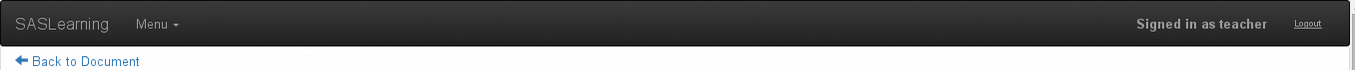
\includegraphics[scale=0.4]{images/header}
\caption{How the header looks when included in a template}
\label{figure:viewsHeaderLooks}
\end{figure}

Another use for this Thymeleaf feature is in the templates defined for the main concepts - View, Scenario, Module, Component and Connector. Each of these templates are defined in separate \textit{$<$section$>$} tags inside a file. This was done because there are other templates where the information about the concepts is included, and it is much easier to include a fragment containing the whole information than writing the code again. 

For example, inside a View template, information about the Elements included in the View must be shown, which is simply a matter of including the template of each element. Other example of the usefulness of these fragments is when showing the structured representation of a document, which consists of showing all the templates of the concepts associated with it. Again, this is as simple as including all the necessary templates.

Figure \ref{figure:viewScenarioTemplate} shows the Scenario template.
\begin{figure}[h]
\centering
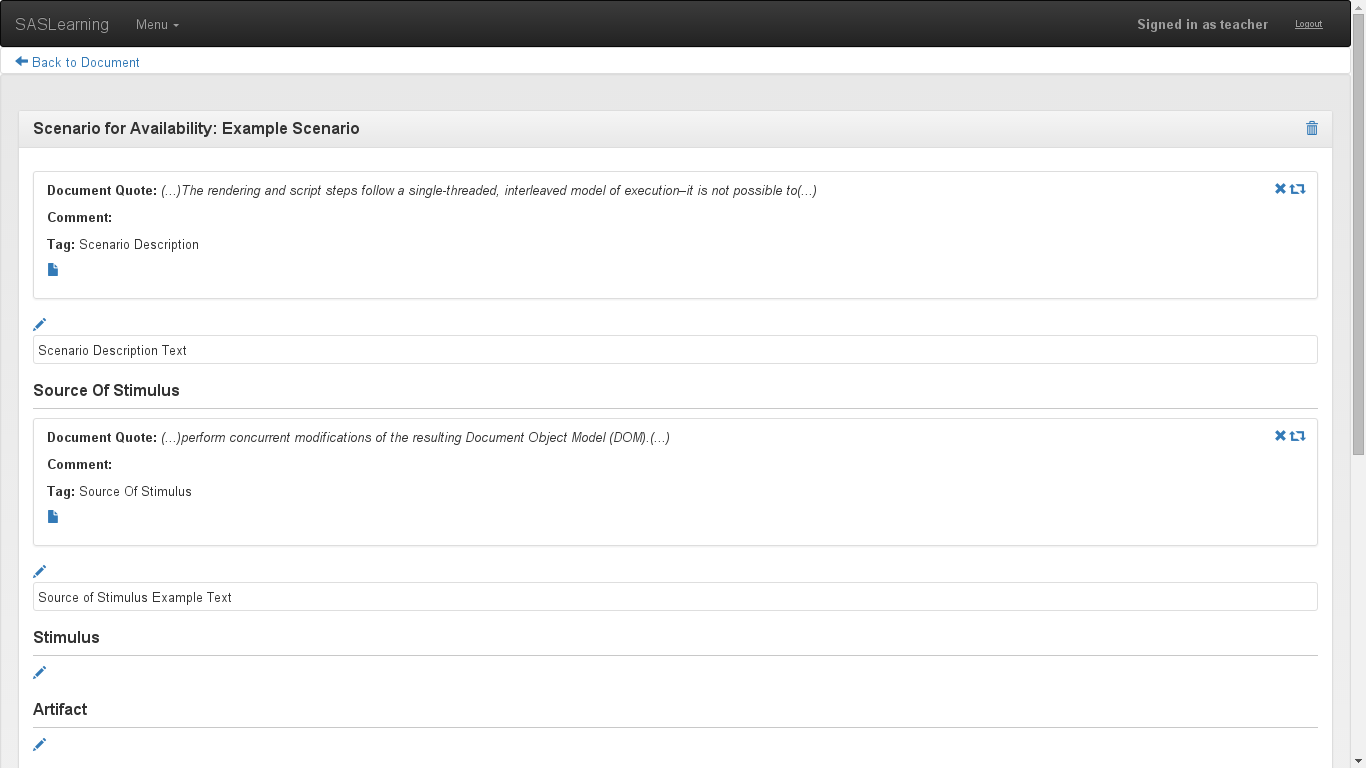
\includegraphics[scale=0.3]{images/scenarioExample}
\caption{Example of the Scenario Template}
\label{figure:viewScenarioTemplate}
\end{figure}
The templates use the information added by the Controllers to the Model Attributes, as seen in Figure \ref{figure:documentControllerStructuredRepresentation} and display it in a structured way. The information added by the Controllers is actually Java objects retrieved from the Model. Thymeleaf allows to treat these attributes as Java objects, so it is possible to obtain the value of the class attributes, or call methods on that object. 

For example, to obtain the Scenario title including the Quality Requirement and the Scenario name as it can be seen in Figure \ref{figure:viewScenarioTemplate}, it is used the Thymeleaf syntax seen in Figure \ref{figure:viewsCallingMethods}. The \textit{\$\{\}} syntax allows to access the variables, and the \textit{th:text} attribute is in fact a Thymeleaf attribute which will set the text inside the \textit{span} tag to the result of the variable access done inside the quotes. As it shown, it is also possible to concatenate the values returned with other static text to obtain the desired results.
\begin{figure}[h]
\centering
\lstset{style=customhtml}
\begin{tabular}{c}
\begin{lstlisting}
<span th:text="'Scenario for '+${scenario.getQualityRequirement().getName()}+': '">
</span> 
<span th:text="${scenario.getName()}"></span>
\end{lstlisting}
\end{tabular}
\caption{How Thymeleaf accesses variables}
\label{figure:viewsCallingMethods}
\end{figure}

Thymeleaf also provides automatic binding of forms information to provided objects. For example, when a user wants to add Modules to a Module Viewtype View, a modal window is prompted, listing all the existent Modules associated with the respective Document, as it is shown in Figure \ref{figure:viewsModalFormExample}. The Modules are listed inside a form, with checkboxes that allow the user to select more than one Module to add. 

\begin{figure}[h]
\centering
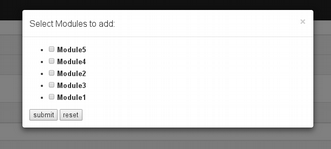
\includegraphics{images/modalExample}
\caption{Example of a Modal window containing a form}
\label{figure:viewsModalFormExample}
\end{figure}

In Figure \ref{figure:ViewControllerViewTemplates}, it is possible to see that the Controller creates and adds a new instance of the \textit{UsedIds} as a model attribute. This instance is used by Thymeleaf to bind the value of the selected checkboxes in the form to the \textit{List$<$String$>$} attribute of the class. Figure \ref{figure:viewFormBindingResult} shows how the form is created.
\begin{figure}[h]
\centering
\lstset{style=customhtml}
\begin{tabular}{c}
\begin{lstlisting}
<form action="#" th:action="@{/addModulesToView/}" method="post">
	<ul>
		<li th:each="module : ${modules}" th:object="${used}">
			<input type="checkbox" th:field="*{used}" 
				th:value="${module.getExternalId()}"></input>
			<label th:text="${module.getName()}"></label>
		</li>
	</ul>
</form>
\end{lstlisting}
\end{tabular}
\caption{Example of a form with object for binding results}
\label{figure:viewFormBindingResult}
\end{figure}
A checkbox is added for each Module in the set. The \textit{th:object} attribute defines that the variable ``used'' is the object to which the results will be bound, and the \textit{th:field} attribute in the \textit{input} tag defines that the value of the checkbox, defined by the \textit{th:value} attribute, if it is chosen, must be bound to the field ``used'' of the class ``UsedIds'', which is the list of type String.

When the form is submitted, Thymeleaf will add the selected values to the list, and send the object in the body of the POST request to the Controller, which will process them as seen in Figure \ref{figure:ViewControllerAddModules}.
					
					













